\documentclass[11pt]{article}
\usepackage[a4paper,margin=0.8in]{geometry}
\usepackage{hyperref}
\usepackage{enumitem}
\usepackage{titlesec}
\usepackage{xcolor}
\usepackage{fancyhdr}
\usepackage{tikz}
\usepackage{graphicx}
\usepackage{eso-pic}

\graphicspath{{../}}

\definecolor{kcpc-bg}{RGB}{250,250,250}
\definecolor{kcpc-text}{RGB}{20,20,20}
\definecolor{kcpc-muted}{RGB}{90,90,90}
\definecolor{kcpc-red}{RGB}{176,0,0}

\pagestyle{fancy}
\fancyhf{}
\lhead{\textcolor{kcpc-text}{\small\bfseries Reading List}}
\rhead{\textcolor{kcpc-muted}{\small Week 1}}
\cfoot{\textcolor{kcpc-muted}{\small KCPC}}
\renewcommand{\headrulewidth}{0.4pt}
\renewcommand{\headrule}{\hbox
to\headwidth{\color{kcpc-red}\leaders\hrule height \headrulewidth\hfill}}
\renewcommand{\footrulewidth}{0pt}
\setlength{\headheight}{28pt}

\AddToShipoutPictureBG{%
    \begin{tikzpicture}[remember picture,overlay]
        \node[opacity=0.035, at=(current page.center)]
        {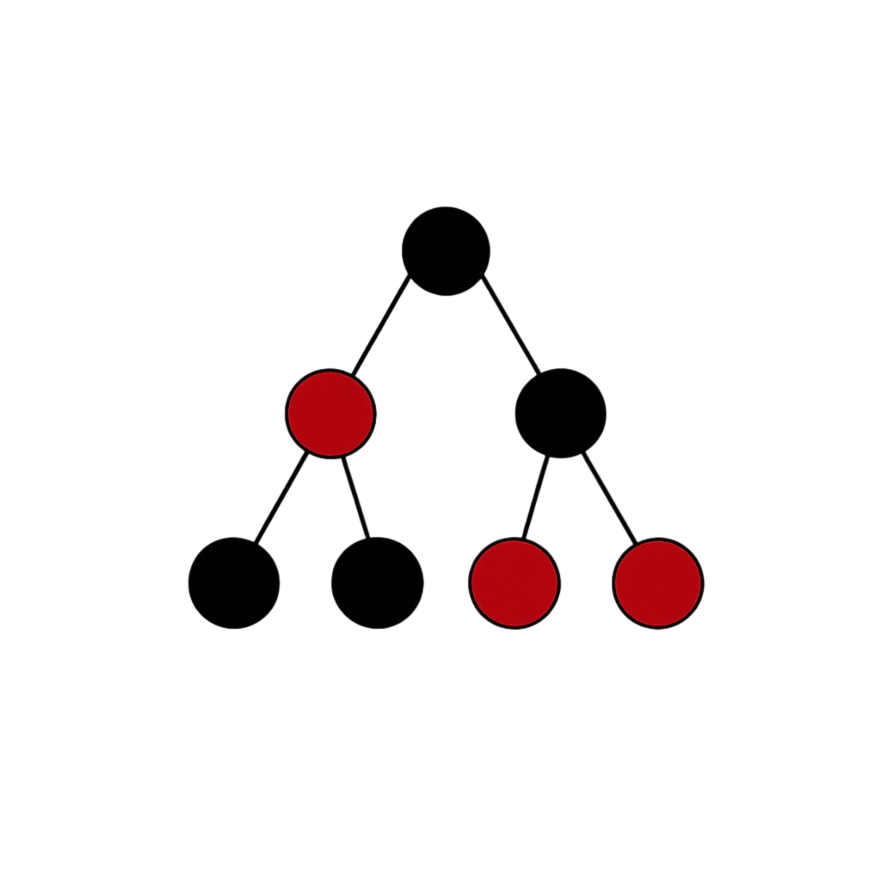
\includegraphics[width=0.38\paperwidth]{kcpc-logo.png}};
    \end{tikzpicture}%
}

\titleformat{\section}{\large\bfseries\color{kcpc-red}}{}{0pt}{}
\titlespacing*{\section}{0pt}{8pt}{2pt}
\setlist[itemize]{leftmargin=*, itemsep=1pt, topsep=2pt}
\setlength{\parindent}{0pt}
\newcommand{\bookentry}[2]{\textbf{#1}\par #2\par\vspace{7pt}}

\title{KCPC Week 1 Reading List\\Reasoning Foundations}
\author{}
\date{}

\begin{document}
\thispagestyle{fancy}

\begin{center}
    {\LARGE\bfseries KCPC Week 1 Reading List}\par
    \vspace{2pt}
    {\large Reasoning Foundations: Logic, Invariants \& Heuristics}
\end{center}
\vspace{5pt}

\bookentry{How to Solve It George P\'olya (Princeton University
Press, 2004)}{A classic introduction to solving unfamiliar problems.
    P\'olya's four-stage method---understand the problem, devise a plan,
    carry it out, and look back---provides a useful routine for every
    puzzle in Week 1. The book develops practical heuristics through
    approachable mathematical examples rather than presenting a catalogue
of formulas.}

\bookentry{The Art and Craft of Problem Solving Paul Zeitz (Wiley,
2007)}{A lively guide to the habits behind successful problem
    solving. Zeitz explores experimentation, pattern recognition,
    symmetry, parity, invariants, contradiction, and extremal arguments.
    It is especially useful for learning how to make progress when a
    problem gives no obvious starting point, and includes many exercises
suitable for ambitious beginners.}

\bookentry{Problem-Solving Strategies Arthur Engel (Springer,
1998)}{A technique-centred collection for readers who want to develop
    beyond isolated tricks. Engel gives substantial attention to
    invariants, colouring, induction, extremal arguments, and the
    pigeonhole principle. The large bank of worked examples makes it
    particularly relevant to the proof-based puzzles and progressively
harder exercises in Week 1.}

\bookentry{Mathematical Puzzles: A Connoisseur's Collection Peter
Winkler (A K Peters, 2004)}{An engaging selection of elegant puzzles
    from combinatorics, probability, geometry, and logic. The problems
    are short to state but often require exactly the kind of decisive
    insight practised in Week 1. Winkler's explanations are concise and
reveal why the central idea works without hiding the creative leap.}

\bookentry{The Moscow Puzzles Boris A. Kordemsky (Dover Publications,
1992)}{A classic collection of recreational problems involving logic,
    parity, counting, arrangements, and geometric constructions. The
    puzzles range from quick observations to challenges requiring
    sustained reasoning. Its informal style makes it easy to browse,
    while the variety encourages readers to decide for themselves which
Week 1 technique might apply.}

\bookentry{Proofs from THE BOOK Martin Aigner and G\"unter M. Ziegler
(Springer, 2018)}{A collection of exceptionally elegant proofs from
    across mathematics. The chapters demonstrate how parity, counting,
    induction, contradiction, and carefully chosen representations can
    produce arguments that are both rigorous and memorable. Not every
    chapter is introductory, but many examples can be enjoyed with
school-level mathematics and curiosity.}

\end{document}
